%! Author = fusel
%! Date = 24.07.21

% Preamble
\documentclass[final]{fhnwreport}
% Packages
\usepackage{amsmath}
\usepackage{lipsum}
\usepackage[german]{babel}
\usepackage{subcaption}


\title{Cloudbasiertes Praxisrufsystem}  %Project Title
\author{IP 5}                      %Document Type => Technical Report, ...

\begin{document}
    \maketitle
    \begin{figure}[h]\label{fig:title}
        
\includegraphics[width=\linewidth]{graphics/wip}\caption[Titlebild]{Titlebild}
    \end{figure}

    \begin{center}
        \renewcommand\arraystretch{2}
        \begin{tabular}{l l}
            Studenten & Joshua Villing, Kevin Zellweger\\
            Fachbetreuer & Daniel Jossen\\
            Auftraggeberin & Daniel Jossen\\
            Studiengang & Informatik\\
            Hochschule & Hochschule für Technik
        \end{tabular}
    \end{center}

    \clearpage


%%---ABSTRACT----------------------------------------------------------------------------
    \thispagestyle{empty}
    \begin{abstract}
Das Abstract ist eine Art Zusammenfassung des ganzen Dokuments. Es gibt einen Einblick in die Aufgabenstellung, wie diese umgesetzt wurde und welches Ergebnis erreicht wurde. Aus diesem Grund wird das Abstract immer ganz am Schluss der Arbeit verfasst. Es besteht aus einem zusammengehörenden Absatz und umfasst ungefähr 10 bis 20 Zeilen.
Formeln, Referenzen oder andere Unterbrechungen haben im Text nichts zu suchen.
Direkt unter dem Abstract folgt eine Liste von drei bis vier Stichworten/Keywords. Diese werden in alphabetischer Reihenfolge aufgelistet und beschreiben das Themengebiet der Arbeit.

\vspace{2ex}

\textbf{Keywords: Anleitung, LaTeX, Thesis, Vorlage}

\vspace{2ex}

\textbf{Management Summary} siehe PF-IK.

\end{abstract}	

\clearpage

\section*{Vorwort}

\lipsum[1-2]

Fakultativ, siehe PF-IK (URL)


%%---TABLE OF CONTENTS-------------------------------------------------------------------
    \pagenumbering{Roman}
    \tableofcontents
    \clearpage

%%---TEXT--------------------------------------------------------------------------------
    \pagenumbering{arabic}
    \section{Einleitung}

\lipsum[3-4]

Einleitungsbeispiele siehe PF-IK (URL)
    \section{Vorgehensweise}

\subsection{Stakeholder}
\begin{itemize}
    \item Daniel Jossen
    \item Kevin Zellweger
    \item Joshua Villing
\end{itemize}
\subsection{Kommunikation}
\begin{itemize}
    \item Teams
    \item OneNote
    \item Github
\end{itemize}
\subsection{Projektplan}
    \section{Anforderungen}

\subsection{Fachlich}
\subsection{Technisch}

    \section{Konzept}

\subsection{Systemarchitektur}

    \subsubsection*{Überblick}

    Für das Cloudbasierte Praxisruf System sehen wir fünf Komponenten vor: 

    \begin{itemize}
        \item Messaging Service
        \item Cloud Service
        \item Mobile Client
        \item Admin UI
        \item VOIP Mediator
    \end{itemize}


    \begin{figure}[H]
    \centering
    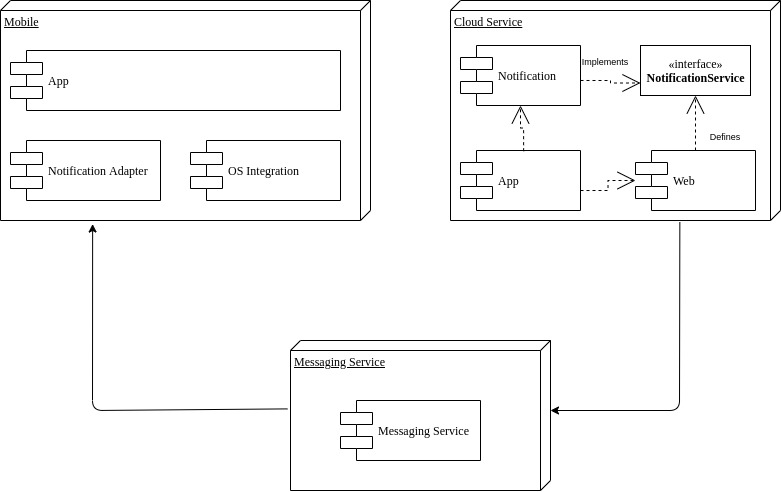
\includegraphics[width=\linewidth]{IP5_POC_Cloud_Architecture.jpg}
    \end{figure}


    \subsubsection*{Mobile Client}

        \begin{itemize}
            \item Der Mobile Client implementiert die Anbindung an den Messaging Service. 
            \item Als Reaktion auf eine Notification wird eine Rückmeldung im UI angezeigt. 
            \item Als Reaktion auf eine Notification wird eine OS Push Notifikation gesendet. 
            Das UI bietet einen Button der eine Anfrage an die REST Schnittstelle im Cloud Service sendet. 
        \end{itemize}


    \subsubsection*{Cloud Service}

        \begin{itemize}
            \item Responsibilities (Notification and Configuration)
            \item Microservice Granularity
        \end{itemize}


    \subsubsection*{Messaging Service}

        \begin{itemize}
            \item Dies wird ein externer Service den wir in die Applikationen einbinden. Standard hierfür ist Firebase Notifications. 
            \item Der Messaging Service nimmt Notifikationen vom Cloud Service entgegen und gibt diese an den Mobile Client wieder. 
            \item Dafür müssen auf beiden Seiten Komponenten eingebaut werden, die mit dem Messaging Service kommunizieren.
        \end{itemize}

\clearpage
\subsection{Mobile Client}
    \subsubsection{Architektur}
    \subsubsection{User Interface}
        \subsubsection*{Home Screen}
            \begin{figure}[H]
            \centering
            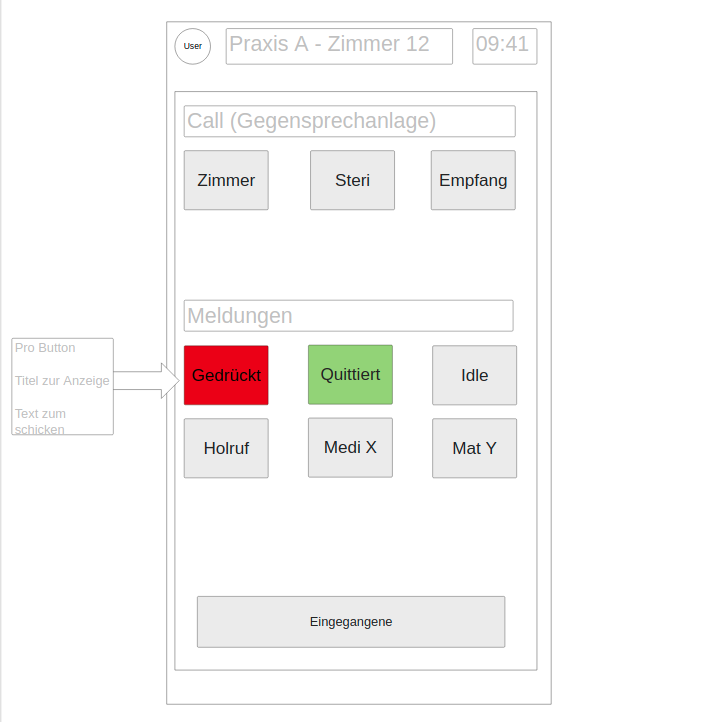
\includegraphics[width=\linewidth]{homescreen-mockup.png}
            \end{figure}
        \subsubsection*{Empfangene Meldungen}
            \begin{figure}[H]
            \centering
            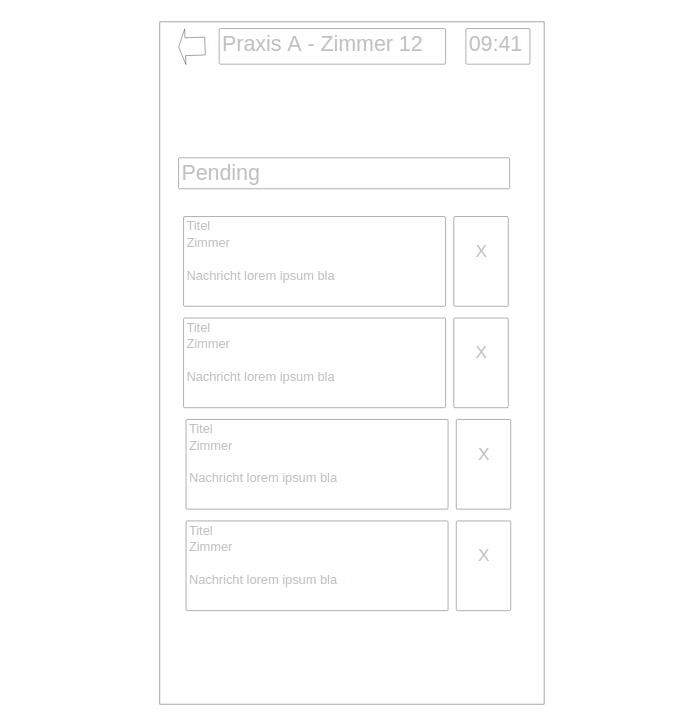
\includegraphics[width=\linewidth]{mockup-received.png}
            \end{figure}


\clearpage
\subsection{Cloud Service}
    \subsubsection{Architektur}
    \subsubsection{Domänenmodell}
    \subsubsection{Laufzeitmodell}

\clearpage
\subsection{Admin UI}

\clearpage
\subsection{Proof Of Concept}
    \subsubsection*{Anforderungen}
        \begin{itemize}
            \item Als <Sender Rolle> möchte ich Notifikationen versenden können. 
            \item Als <Empfänger Rolle> möchte ich Notifikationen in der Applikation sehen, wenn die Applikation geöffnet ist.  
            \item Als <Empfänger Rolle> möchte ich Notifikationen über das OS erhalten, wenn die Applikation minimiert ist. 
        \end{itemize}
    \subsubsection*{Restriktionen}
        \begin{itemize}
            \item Nur 1 Client. 
            \item Nur 1 fixe Notifikation. Keine Types. 
            \item Notifikation wird vom Client gesendet und vom selben Client empfangen. 
            \item Keine Authentication oder Authorization. 
        \end{itemize}

    \section{Evaluation Technologien}

\subsection{Mobile Client}



\url{https://kotlinlang.org/lp/mobile/}
	

    +Jet Brains Infrastructure 
    +We like Kotlin 

    -IoS Env. Needed to develop for Apple 
    -Still has to develop separate API und UI Modules for Platforms 

\url{https://web.dev/progressive-web-apps/ }
	
    +No need of Native Codebase
    +Perfect for Android 
    -Eventually drawbacks because no entire API Access 
    -PWAs on IOS suck

\url{https://cordova.apache.org/} 
	

    + Popular Framework 
    + Tons of plugins to access apis 

    -Still need to have a Mac for IoS development  
    -Not a truly native app -> API Issues
 

\url{https://nativescript.org/ }

    +Provides a Workaround for nasty X-tools 
    +Claims to be truly Native 
    -Do we really trust it? (sorta new and passion project of a few people) 

 
 \url{https://flutter.dev}

    -Why do you hate me?


"Simply Write Everything twice"

    +Would definitely work

    -Do most things twice
    -We don't have time for that
    -Kunde wünscht ausdrücklich nur eine Codebasis für beide Clients.
	

  

\url{https://stackshare.io/stackups/apache-cordova-vs-nativescript 

\url{https://nativescript.org/blog/build-nativescript-apps-remotely-from-windows-or-linux/ }

\subsection{Cloud Service}

    \url{https://aws.amazon.com/  }

    \url{https://spring.io/projects/spring-boot } 

    Konfig der Clients könnte sich als No-SQL anbieten.   

    Config muss nur gelesen und an den Client geschickt oder abgespeichert werden  

    \url{https://www.mongodb.com/}  

  

\subsection{Betrieb und Platform}

AWS ist MUSS
    \section{Umsetzung}
    \section {Schluss}


%%---APPENDIX----------------------------------------------------------------------------
    \begin{appendix} %Anhang
\section{Ein Anhang}

\lipsum[61-64]

%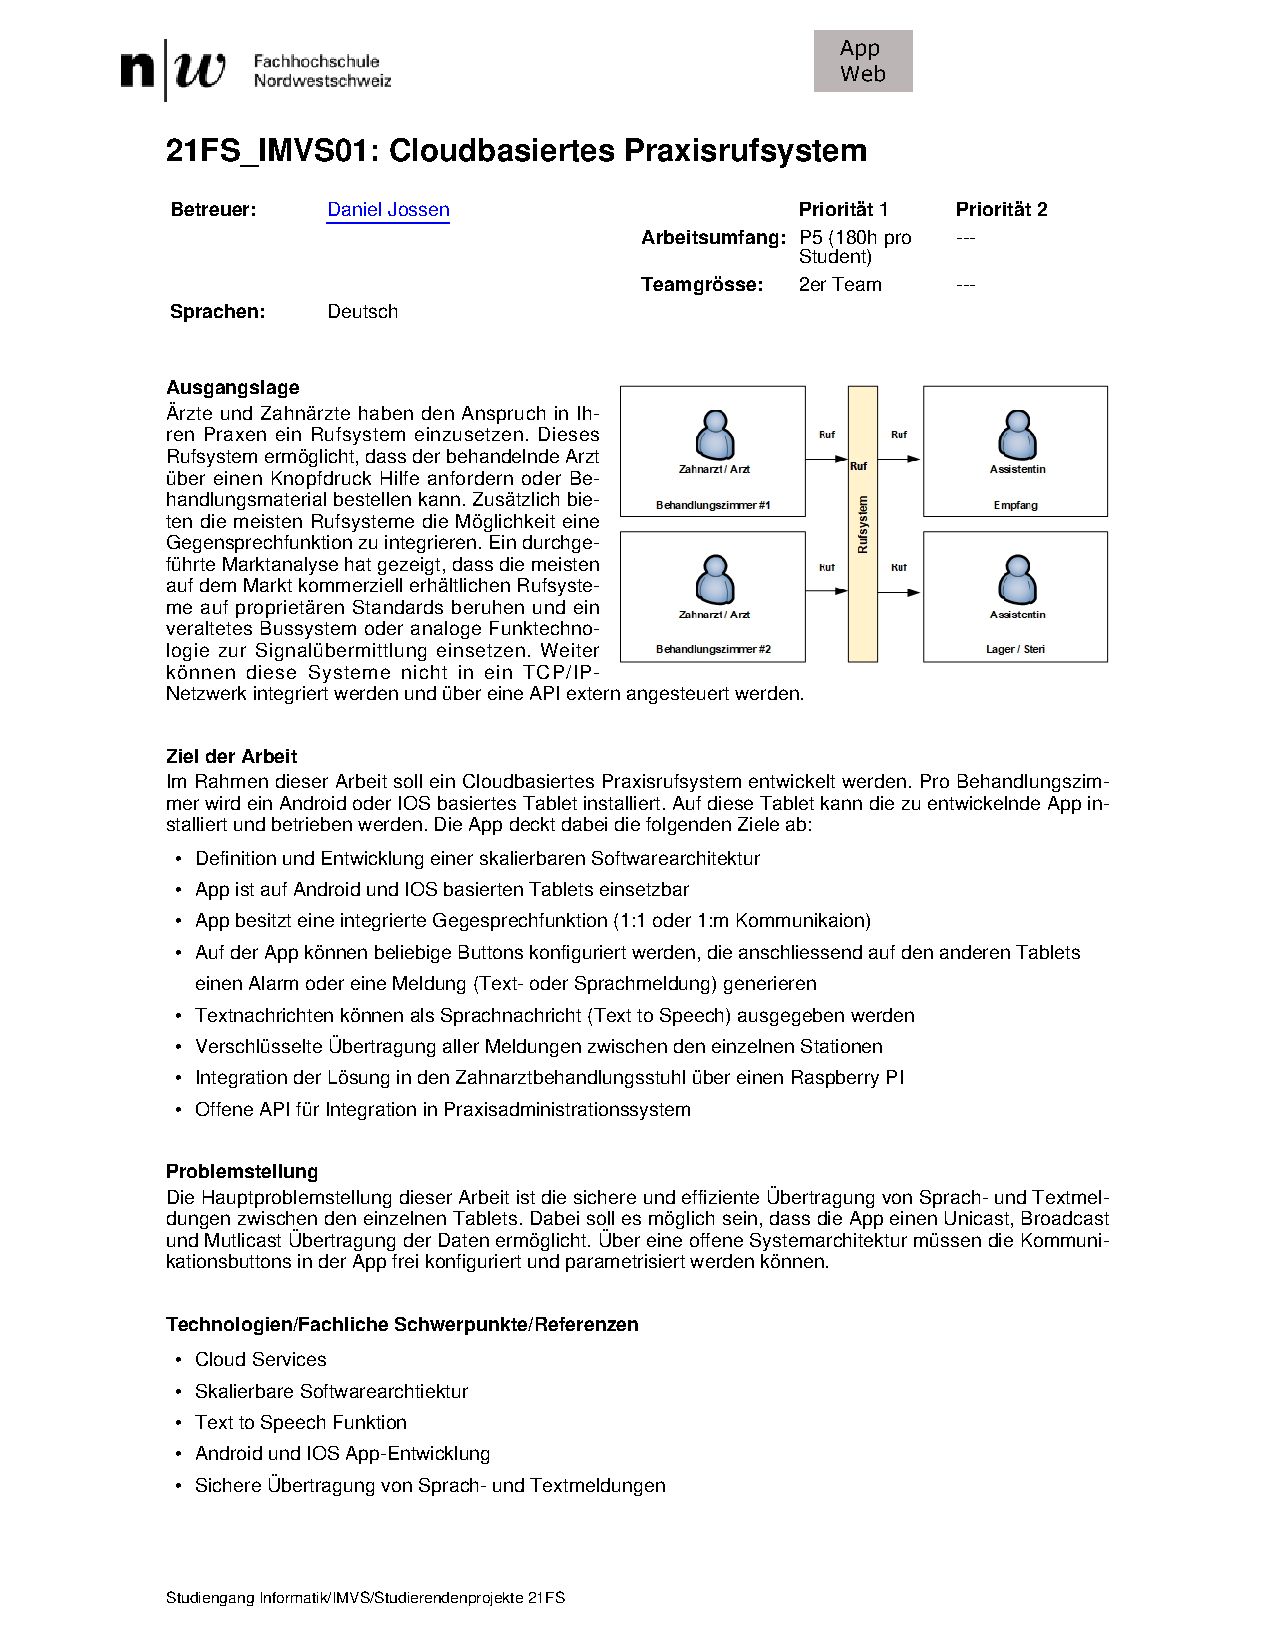
\includepdf[pages={1-2},nup=1x2,landscape=true,scale=0.85,offset=10 -40,pagecommand={\section{Eingefügtes Dokument; zwei Seiten auf einer}\label{app:Aufgabenstellung}\thispagestyle{myheadings}}]{appendix/aufgabenstellung.pdf} \newpage

%%Bei mehrseitigen Dokumenten die folgenden Seiten ohne Überschrift:
%\includepdf[pages={3-6},nup=1x2,landscape=true,scale=0.85,offset=10 -40,pagecommand={\thispagestyle{myheadings}}]{appendix/aufgabenstellung.pdf} \newpage

%\includepdf[pages={1},nup=1x1,landscape=true,scale=0.85,offset=10 -40,pagecommand={\section{Eingefügte PDF-Tabelle}\label{app:Timetable}\thispagestyle{myheadings}}]{appendix/timeline_example.pdf} \newpage

%%Bei mehrseitigen Dokumenten die folgenden Seiten ohne Überschrift:
%\includepdf[pages={2-5},nup=1x1,landscape=true,scale=0.85,offset=0 -20,pagecommand={\thispagestyle{myheadings}}]{appendix/timeline_example.pdf} \newpage

\end{appendix}


\end{document}
